\section{Hyperparameter tuning}

The online scheduling algorithm cluster genotype has a handful of hyperparameters. They are all shown in the table \ref{tab:hyper_all}, along with their values which we will consider. One of the hyperparameters is the optimization algorithm which is used for training, and each algorithm has several hyperparameters.

For the topology partitioner scheme, the number $k$ is calculated as the mathematical round of the square root of the total number of elements in the topology which require an online scheduling algorithm.

\begin{table}[!htbp]
    \begin{center}
        \begin{tabular}{|>{\raggedright\arraybackslash}p{0.3\linewidth}|>{\raggedright\arraybackslash}p{0.6\linewidth}|} 
         \hline
            Hyperparameter & Values \\ [0.5ex] \hline\hline
            cluster combination operator granularity & coarse, fine \\
            \hline
            topology partitioner scheme & all, 1 beginning, 1 end, 1 fair random, 1 true random, k beginning, k end, k fair random, k true random, random path \\
            \hline
            random path topology enumerator change element chance & 0.5, 0.6, 0.7, 0.8, 0.9 \\
            \hline
            optimization algorithm & SSGA, GGA, ES, SIA, CLONALG \\
            \hline
            SSGA population size & 5, 10, 15, 20 \\
            \hline
            SSGA evaluations in inner algorithm & 100, 50, 25, 20 \\
            \hline
            GGA population size & 5, 10, 15, 20 \\
            \hline
            GGA evaluations in inner algorithm & 100, 50, 25, 20 \\
            \hline
            GGA worst unit coefficient & 0.1, 0.2, 0.3, 0.4, 0.5 \\
            \hline
            ES population size & 5, 10, 15, 20 \\
            \hline
            ES evaluations in inner algorithm & 100, 50, 25, 20 \\
            \hline
            ES new units per generation percentage & 0.05, 0.1, 0.15, 0.2, 0.3, 0.4, 0.5 \\
            \hline
            SIA population size & 5, 10, 15, 20 \\
            \hline
            SIA evaluations in inner algorithm & 100, 50, 25, 20 \\
            \hline
            SIA number of clones per individual & 1, 2, 3, 4, 5 \\
            \hline
            CLONALG population size & 5, 10, 15, 20 \\
            \hline
            CLONALG evaluations in inner algorithm & 100, 50, 25, 20 \\
            \hline
            CLONALG $\beta$ & 0.1, 0.2, 0.3, 0.4, 0.5 \\
            \hline
            CLONALG $\gamma$ & 0.05, 0.1, 0.15, 0.2 \\
            \hline
            CLONALG $\lambda$ & 3, 5, 8, 10 \\
            \hline
        \end{tabular}
    \end{center}
    \caption{Hyperparameter values - all algorithms}
\label{tab:hyper_all}
\end{table}

Furthermore, the online scheduling algorithm cluster has an additional parameter, which is the online scheduling algorithm it employs for all regression problems. Each online scheduling algorithm has several hyperparameters. They are shown in the following tables - NN in table \ref{tab:hyper_nn}, TBGP in table \ref{tab:hyper_tbgp}, CGP in table \ref{tab:hyper_cgp}, GBGP in table \ref{tab:hyper_gbgp}, SBGP in table \ref{tab:hyper_sbgp}, LGP in table \ref{tab:hyper_lgp}, MEP in table \ref{tab:hyper_mep}, GEP in table \ref{tab:hyper_gep}, GE in table \ref{tab:hyper_ge} and SGE in table \ref{tab:hyper_sge}.

\begin{table}[!htbp]
    \begin{center}
        \begin{tabular}{|>{\raggedright\arraybackslash}p{0.3\linewidth}|>{\raggedright\arraybackslash}p{0.6\linewidth}|} 
         \hline
            Hyperparameter & Values \\ [0.5ex] \hline\hline
            creation $\sigma$ & 0.001, 0.01, 0.1, 1.0 \\
            \hline
            perturbation $\sigma$ & 0.001, 0.01, 0.1, 1.0 \\
            \hline
            activation function & sigmoid, ReLU, tanh, leaky ReLU \\
            \hline
            hidden layers & $-$, $5$, $10$, $20$, $10 \times 5$, $10 \times 10$, $20 \times 10$, $20 \times 20$, $10 \times 10 \times 5$, $20 \times 10 \times 5$, $20 \times 20 \times 20$, $20 \times 15 \times 10 \times 5$ \\
            \hline
        \end{tabular}
    \end{center}
    \caption{Hyperparameter values - NN}
\label{tab:hyper_nn}
\end{table}

\begin{table}[!htbp]
    \begin{center}
        \begin{tabular}{|>{\raggedright\arraybackslash}p{0.3\linewidth}|>{\raggedright\arraybackslash}p{0.6\linewidth}|} 
         \hline
            Hyperparameter & Values \\ [0.5ex] \hline\hline
            maximum height & 5, 8, 10, 12, 15 \\
            \hline
            constant leaf chance & 0.05, 0.1, 0.15, 0.2\\
            \hline
            parameter leaf chance & 0.1, 0.2, 0.3, 0.4, 0.5 \\
            \hline
        \end{tabular}
    \end{center}
    \caption{Hyperparameter values - TBGP}
\label{tab:hyper_tbgp}
\end{table}

\begin{table}[!htbp]
    \begin{center}
        \begin{tabular}{|>{\raggedright\arraybackslash}p{0.3\linewidth}|>{\raggedright\arraybackslash}p{0.6\linewidth}|} 
         \hline
            Hyperparameter & Values \\ [0.5ex] \hline\hline
            number of rows & 3, 5, 8, 10, 15 \\
            \hline
            number of columns & 3, 5, 8, 10, 15 \\
            \hline
            perturbation rate & 0.05, 0.1, 0.2, 0.3 \\
            \hline
        \end{tabular}
    \end{center}
    \caption{Hyperparameter values - CGP}
\label{tab:hyper_cgp}
\end{table}

\begin{table}[!htbp]
    \begin{center}
        \begin{tabular}{|>{\raggedright\arraybackslash}p{0.3\linewidth}|>{\raggedright\arraybackslash}p{0.6\linewidth}|} 
         \hline
            Hyperparameter & Values \\ [0.5ex] \hline\hline
            maximum number of nodes & 20, 50, 100, 150, 200, 300 \\
            \hline
            perturbation rate & 0.05, 0.1, 0.2, 0.3 \\
            \hline
            maximum nodes to delete & 1, 2, 3, 4, 5 \\
            \hline
            maximum nodes to insert & 1, 2, 3, 4, 5 \\
            \hline
            maximum nodes in crossover & 5, 10, 15, 20 \\
            \hline
            exchange branch in crossover chance & 0.5, 0.6, 0.7, 0.8, 0.9 \\
            \hline
        \end{tabular}
    \end{center}
    \caption{Hyperparameter values - GBGP}
\label{tab:hyper_gbgp}
\end{table}

\begin{table}[!htbp]
    \begin{center}
        \begin{tabular}{|>{\raggedright\arraybackslash}p{0.3\linewidth}|>{\raggedright\arraybackslash}p{0.6\linewidth}|} 
         \hline
            Hyperparameter & Values \\ [0.5ex] \hline\hline
            number of instructions & 20, 50, 100, 150, 200, 300 \\
            \hline
            creation chance of NOP & 0.1, 0.2, 0.3, 0.4, 0.5 \\
            \hline
            perturbation chance of NOP & 0.1, 0.2, 0.3, 0.4, 0.5 \\
            \hline
            PUSH constant share & 0.1, 0.2, 0.3 \\
            \hline
            PUSH param share & 0.1, 0.2, 0.3, 0.4, 0.5 \\
            \hline
            perturbation rate & 0.05, 0.1, 0.2, 0.3 \\
            \hline
        \end{tabular}
    \end{center}
    \caption{Hyperparameter values - SBGP}
\label{tab:hyper_sbgp}
\end{table}

\begin{table}[!htbp]
    \begin{center}
        \begin{tabular}{|>{\raggedright\arraybackslash}p{0.3\linewidth}|>{\raggedright\arraybackslash}p{0.6\linewidth}|} 
         \hline
            Hyperparameter & Values \\ [0.5ex] \hline\hline
            register initialization strategy & empty, singular, circular \\
            \hline
            number of registers & 5, 10, 15, 20 \\
            \hline
            number of instructions & 20, 50, 100, 150, 200, 300 \\
            \hline
            creation chance of NOP & 0.1, 0.2, 0.3, 0.4, 0.5 \\
            \hline
            perturbation chance of NOP & 0.1, 0.2, 0.3, 0.4, 0.5 \\
            \hline
            perturbation rate & 0.05, 0.1, 0.2, 0.3 \\
            \hline
        \end{tabular}
    \end{center}
    \caption{Hyperparameter values - LGP}
\label{tab:hyper_lgp}
\end{table}

\begin{table}[!htbp]
    \begin{center}
        \begin{tabular}{|>{\raggedright\arraybackslash}p{0.3\linewidth}|>{\raggedright\arraybackslash}p{0.6\linewidth}|} 
         \hline
            Hyperparameter & Values \\ [0.5ex] \hline\hline
            number of instructions & 20, 50, 100, 150, 200, 300 \\
            \hline
            perturbation rate & 0.05, 0.1, 0.2, 0.3 \\
            \hline
        \end{tabular}
    \end{center}
    \caption{Hyperparameter values - MEP}
\label{tab:hyper_mep}
\end{table}

\begin{table}[!htbp]
    \begin{center}
        \begin{tabular}{|>{\raggedright\arraybackslash}p{0.3\linewidth}|>{\raggedright\arraybackslash}p{0.6\linewidth}|} 
         \hline
            Hyperparameter & Values \\ [0.5ex] \hline\hline
            head size & 10, 20, 30, 40, 50 \\
            \hline
            tail chance of parameter & 0.5, 0.6, 0.7, 0.8, 0.9 \\
            \hline
            perturbation rate & 0.05, 0.1, 0.2, 0.3 \\
            \hline
            chance of transposition & 0.2, 0.4, 0.5, 0.6, 0.8 \\
            \hline
            maximum length of transposition & 2, 5, 8, 10, 15, 20 \\
            \hline
        \end{tabular}
    \end{center}
    \caption{Hyperparameter values - GEP}
\label{tab:hyper_gep}
\end{table}

\begin{table}[!htbp]
    \begin{center}
        \begin{tabular}{|>{\raggedright\arraybackslash}p{0.3\linewidth}|>{\raggedright\arraybackslash}p{0.6\linewidth}|} 
         \hline
            Hyperparameter & Values \\ [0.5ex] \hline\hline
            number of codons & 20, 50, 100, 150, 200, 300 \\
            \hline
            maximum number of wrappings & 0, 1, 2, 3, 4, 5 \\
            \hline
            perturbation rate & 0.05, 0.1, 0.2, 0.3 \\
            \hline
        \end{tabular}
    \end{center}
    \caption{Hyperparameter values - GE}
\label{tab:hyper_ge}
\end{table}

\begin{table}[!htbp]
    \begin{center}
        \begin{tabular}{|>{\raggedright\arraybackslash}p{0.3\linewidth}|>{\raggedright\arraybackslash}p{0.6\linewidth}|} 
         \hline
            Hyperparameter & Values \\ [0.5ex] \hline\hline
            maximum depth & 3, 4, 5 \\
            \hline
            perturbation rate & 0.05, 0.1, 0.2, 0.3 \\
            \hline
        \end{tabular}
    \end{center}
    \caption{Hyperparameter values - SGE}
\label{tab:hyper_sge}
\end{table}

Figure \ref{fig:experiment0_topology} shows the topology which was used for tuning hyperparameters. The train job sequence had $50$ jobs, and the test job sequence had $100$ jobs.

\begin{figure}[!htbp]
	\centering
	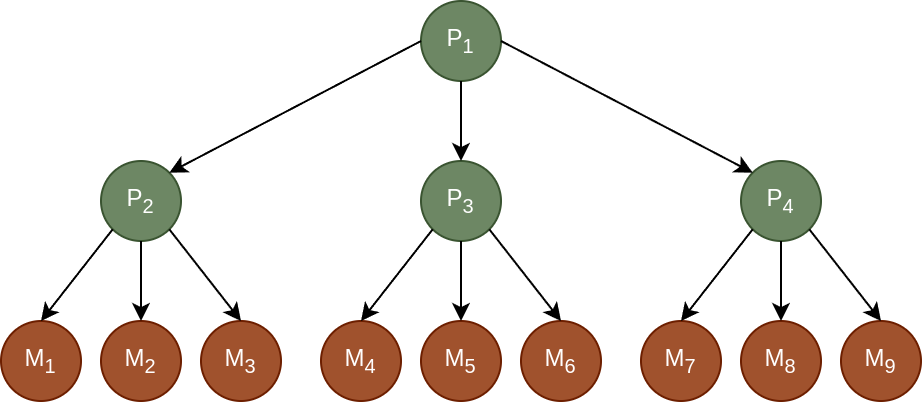
\includegraphics[scale=0.6]{../images/experiment0_topology.png}
	\caption{Experiment 0 - topology}
    \label{fig:experiment0_topology}
\end{figure}

While most of the hyperparameters were transferred from the tuning process directly to the experiments, some of them were scaled. The motivation behind this was to test as many hyperparameter configurations as possible in a limited time, and the hyperparameters which affect complexity the most were scaled down. Table \ref{tab:hyper_scale_population} shows how the population size was scaled, and the table \ref{tab:hyper_scale_evaluations} shows how the number of evaluations was scaled. In the second table, the notation $x/y$ means the following - the loop in the scheduling meta algorithm has $x$ iterations, while the inner optimization algorithm has $y$ evaluations of the evaluation function for the genotype. The goal here was to try to find a good ratio between these two values, while keeping the total number of evaluations of the evaluation function constant.

\begin{table}[!htbp]
    \begin{center}
        \begin{tabular}{|l|l|} 
         \hline
            Old value & New value \\ [0.5ex] \hline\hline
            5 & 50 \\
            \hline
            10 & 100 \\
            \hline
            15 & 150 \\
            \hline
            20 & 200 \\
            \hline
        \end{tabular}
    \end{center}
    \caption{Hyperparameter values - scaling population size}
\label{tab:hyper_scale_population}
\end{table}

\begin{table}[!htbp]
    \begin{center}
        \begin{tabular}{|l|l|} 
         \hline
            Old values & New values \\ [0.5ex] \hline\hline
            10/100 & 50/1000 \\
            \hline
            20/50 & 100/500 \\
            \hline
            40/25 & 200/250 \\
            \hline
            50/20 & 500/100 \\
            \hline
        \end{tabular}
    \end{center}
    \caption{Hyperparameter values - scaling number of evaluations}
\label{tab:hyper_scale_evaluations}
\end{table}

The hyperparameters were tuned for each algorithm separately. This could not be solved using an exhaustive method such as the grid search, as there are too many possible hyperparameter configurations for each algorithm. Instead, the problem was framed as an optimization problem, and the algorithm which was used for optimization was SSGA. A similar approach, used for tuning hyperparameters for machine learning models, can be found in \citep{hyperopti}.

The genotype for this problem was the mapping from hyperparameters to their values. The evaluation function would take these hyperparameters and try to solve the problem of creating a good online scheduling system. In other words, the evaluation function was the execution of the scheduling meta algorithm. The creation operator would generate a random value for each hyperparameter. The combination operator would, for each hyperparameter, randomly choose one of the two parents and copy its value for the hyperparameter. The perturbation operator would randomly select some hyperparameters and change their values. The hyperparameters of the SSGA used for tuning hyperparameters were the following - population size was $10$, number of evaluations of the evaluation function was $200$, and the perturbation rate was $0.2$.

Results of the hyperparameter tuning for online scheduling algorithms are shown in the following tables - NN in table \ref{tab:hyper_nn_results}, 
TBGP in table \ref{tab:hyper_tbgp_results}, CGP in table \ref{tab:hyper_cgp_results}, GBGP in table \ref{tab:hyper_gbgp_results}, SBGP in table \ref{tab:hyper_sbgp_results}, LGP in table \ref{tab:hyper_lgp_results}, MEP in table \ref{tab:hyper_mep_results}, GEP in table \ref{tab:hyper_gep_results}, GE in table \ref{tab:hyper_ge_results} and SGE in table \ref{tab:hyper_sge_results}.

\begin{table}[!htbp]
    \centering
    \resizebox{\textwidth}{!}{
        \begin{tabular}{|l|l|l|l|l|l|l|l|l|l|l|l|}
        \hline
        Hyperparameter & Value \\ [0.5ex] \hline\hline
        cluster combination operator granularity & fine \\
        \hline
        topology partitioner scheme & k true random \\
        \hline
        random path topology enumerator change element chance & 0.6 \\
        \hline
        optimization algorithm & SIA \\
        \hline
        SSGA population size & 5 \\
        \hline
        SSGA evaluations in inner algorithm & 100 \\
        \hline
        GGA population size & 15 \\
        \hline
        GGA evaluations in inner algorithm & 100 \\
        \hline
        GGA worst unit coefficient & 0.1 \\
        \hline
        ES population size & 5 \\
        \hline
        ES evaluations in inner algorithm & 20 \\
        \hline
        ES new units per generation percentage & 0.5 \\
        \hline
        SIA population size & 15 \\
        \hline
        SIA evaluations in inner algorithm & 20 \\
        \hline
        SIA number of clones per individual & 5 \\
        \hline
        CLONALG population size & 15 \\
        \hline
        CLONALG evaluations in inner algorithm & 25 \\
        \hline
        CLONALG $\beta$ & 0.1 \\
        \hline
        CLONALG $\gamma$ & 0.2 \\
        \hline
        CLONALG $\lambda$ & 8 \\
        \hline
        creation $\sigma$ & 0.001 \\
        \hline
        perturbation $\sigma$ & 0.01 \\
        \hline
        activation function & sigmoid \\
        \hline
        hidden layers & $5$ \\
        \hline
        \end{tabular}
    }
    \caption{Hyperparameter tuning results - NN}
    \label{tab:hyper_nn_results}
\end{table}

\begin{table}[!htbp]
    \centering
    \resizebox{\textwidth}{!}{
        \begin{tabular}{|l|l|l|l|l|l|l|l|l|l|l|l|}
        \hline
        Hyperparameter & Value \\ [0.5ex] \hline\hline
        cluster combination operator granularity & fine \\
        \hline
        topology partitioner scheme & k true random \\
        \hline
        random path topology enumerator change element chance & 0.5 \\
        \hline
        optimization algorithm & SSGA \\
        \hline
        SSGA population size & 20 \\
        \hline
        SSGA evaluations in inner algorithm & 20 \\
        \hline
        GGA population size & 10 \\
        \hline
        GGA evaluations in inner algorithm & 20 \\
        \hline
        GGA worst unit coefficient & 0.5 \\
        \hline
        ES population size & 20 \\
        \hline
        ES evaluations in inner algorithm & 25 \\
        \hline
        ES new units per generation percentage & 0.15 \\
        \hline
        SIA population size & 10 \\
        \hline
        SIA evaluations in inner algorithm & 25 \\
        \hline
        SIA number of clones per individual & 4 \\
        \hline
        CLONALG population size & 20 \\
        \hline
        CLONALG evaluations in inner algorithm & 20 \\
        \hline
        CLONALG $\beta$ & 0.5 \\
        \hline
        CLONALG $\gamma$ & 0.15\\
        \hline
        CLONALG $\lambda$ & 10 \\
        \hline
        maximum height & 10 \\
        \hline
        constant leaf chance & 0.05 \\
        \hline
        parameter leaf chance & 0.3 \\
        \hline
        \end{tabular}
    }
    \caption{Hyperparameter tuning results - TBGP}
    \label{tab:hyper_tbgp_results}
\end{table}

\begin{table}[!htbp]
    \centering
    \resizebox{\textwidth}{!}{
        \begin{tabular}{|l|l|l|l|l|l|l|l|l|l|l|l|}
        \hline
        Hyperparameter & Value \\ [0.5ex] \hline\hline
        cluster combination operator granularity & fine \\
        \hline
        topology partitioner scheme & all \\
        \hline
        random path topology enumerator change element chance & 0.6 \\
        \hline
        optimization algorithm & SSGA \\
        \hline
        SSGA population size & 10 \\
        \hline
        SSGA evaluations in inner algorithm & 100 \\
        \hline
        GGA population size & 15 \\
        \hline
        GGA evaluations in inner algorithm & 20 \\
        \hline
        GGA worst unit coefficient & 0.2 \\
        \hline
        ES population size & 5 \\
        \hline
        ES evaluations in inner algorithm & 100 \\
        \hline
        ES new units per generation percentage & 0.4 \\
        \hline
        SIA population size & 5 \\
        \hline
        SIA evaluations in inner algorithm & 25 \\
        \hline
        SIA number of clones per individual & 2 \\
        \hline
        CLONALG population size & 15 \\
        \hline
        CLONALG evaluations in inner algorithm & 50 \\
        \hline
        CLONALG $\beta$ & 0.3 \\
        \hline
        CLONALG $\gamma$ & 0.1 \\
        \hline
        CLONALG $\lambda$ & 10 \\
        \hline
        number of rows & 15 \\
        \hline
        number of columns & 15 \\
        \hline
        perturbation rate & 0.05 \\
        \hline
        \end{tabular}
    }
    \caption{Hyperparameter tuning results - CGP}
    \label{tab:hyper_cgp_results}
\end{table}

\begin{table}[!htbp]
    \centering
    \resizebox{\textwidth}{!}{
        \begin{tabular}{|l|l|l|l|l|l|l|l|l|l|l|l|}
        \hline
        Hyperparameter & Value \\ [0.5ex] \hline\hline
        cluster combination operator granularity & fine \\
        \hline
        topology partitioner scheme & random path \\
        \hline
        random path topology enumerator change element chance & 0.8 \\
        \hline
        optimization algorithm & SSGA \\
        \hline
        SSGA population size & 15 \\
        \hline
        SSGA evaluations in inner algorithm & 50 \\
        \hline
        GGA population size & 10 \\
        \hline
        GGA evaluations in inner algorithm & 20 \\
        \hline
        GGA worst unit coefficient & 0.2 \\
        \hline
        ES population size & 15 \\
        \hline
        ES evaluations in inner algorithm & 20 \\
        \hline
        ES new units per generation percentage & 0.05 \\
        \hline
        SIA population size & 5 \\
        \hline
        SIA evaluations in inner algorithm & 25 \\
        \hline
        SIA number of clones per individual & 2 \\
        \hline
        CLONALG population size & 15 \\
        \hline
        CLONALG evaluations in inner algorithm & 25 \\
        \hline
        CLONALG $\beta$ & 0.2 \\
        \hline
        CLONALG $\gamma$ & 0.1 \\
        \hline
        CLONALG $\lambda$ & 3 \\
        \hline
        maximum number of nodes & 300 \\
        \hline
        perturbation rate & 0.2 \\
        \hline
        maximum nodes to delete & 1 \\
        \hline
        maximum nodes to insert & 4 \\
        \hline
        maximum nodes in crossover & 10 \\
        \hline
        exchange branch in crossover chance & 0.6 \\
        \hline
        \end{tabular}
    }
    \caption{Hyperparameter tuning results - GBGP}
    \label{tab:hyper_gbgp_results}
\end{table}

\begin{table}[!htbp]
    \centering
    \resizebox{\textwidth}{!}{
        \begin{tabular}{|l|l|l|l|l|l|l|l|l|l|l|l|}
        \hline
        Hyperparameter & Value \\ [0.5ex] \hline\hline
        cluster combination operator granularity & coarse \\
        \hline
        topology partitioner scheme & random path \\
        \hline
        random path topology enumerator change element chance & 0.9 \\
        \hline
        optimization algorithm & ES \\
        \hline
        SSGA population size & 20 \\
        \hline
        SSGA evaluations in inner algorithm & 20 \\
        \hline
        GGA population size & 20 \\
        \hline
        GGA evaluations in inner algorithm & 100 \\
        \hline
        GGA worst unit coefficient & 0.5 \\
        \hline
        ES population size & 20 \\
        \hline
        ES evaluations in inner algorithm & 50 \\
        \hline
        ES new units per generation percentage & 0.3 \\
        \hline
        SIA population size & 5 \\
        \hline
        SIA evaluations in inner algorithm & 25 \\
        \hline
        SIA number of clones per individual & 3 \\
        \hline
        CLONALG population size & 10 \\
        \hline
        CLONALG evaluations in inner algorithm & 100 \\
        \hline
        CLONALG $\beta$ & 0.1 \\
        \hline
        CLONALG $\gamma$ & 0.15 \\
        \hline
        CLONALG $\lambda$ & 5 \\
        \hline
        number of instructions & 200 \\
        \hline
        creation chance of NOP & 0.3 \\
        \hline
        perturbation chance of NOP & 0.2 \\
        \hline
        PUSH constant share & 0.1 \\
        \hline
        PUSH param share & 0.3 \\
        \hline
        perturbation rate & 0.3 \\
        \hline
        \end{tabular}
    }
    \caption{Hyperparameter tuning results - SBGP}
    \label{tab:hyper_sbgp_results}
\end{table}

\begin{table}[!htbp]
    \centering
    \resizebox{\textwidth}{!}{
        \begin{tabular}{|l|l|l|l|l|l|l|l|l|l|l|l|}
        \hline
        Hyperparameter & Value \\ [0.5ex] \hline\hline
        cluster combination operator granularity & fine \\
        \hline
        topology partitioner scheme & random path \\
        \hline
        random path topology enumerator change element chance & 0.9 \\
        \hline
        optimization algorithm & ES \\
        \hline
        SSGA population size & 15 \\
        \hline
        SSGA evaluations in inner algorithm & 100 \\
        \hline
        GGA population size & 15 \\
        \hline
        GGA evaluations in inner algorithm & 50 \\
        \hline
        GGA worst unit coefficient & 0.1 \\
        \hline
        ES population size & 5 \\
        \hline
        ES evaluations in inner algorithm & 20 \\
        \hline
        ES new units per generation percentage & 0.3 \\
        \hline
        SIA population size & 10 \\
        \hline
        SIA evaluations in inner algorithm & 100 \\
        \hline
        SIA number of clones per individual & 5 \\
        \hline
        CLONALG population size & 20 \\
        \hline
        CLONALG evaluations in inner algorithm & 25 \\
        \hline
        CLONALG $\beta$ & 0.3 \\
        \hline
        CLONALG $\gamma$ & 0.2 \\
        \hline
        CLONALG $\lambda$ & 5 \\
        \hline
        register initialization strategy & singular \\
        \hline
        number of registers & 10 \\
        \hline
        number of instructions & 100 \\
        \hline
        creation chance of NOP & 0.3 \\
        \hline
        perturbation chance of NOP & 0.4 \\
        \hline
        perturbation rate & 0.05 \\
        \hline
        \end{tabular}
    }
    \caption{Hyperparameter tuning results - LGP}
    \label{tab:hyper_lgp_results}
\end{table}

\begin{table}[!htbp]
    \centering
    \resizebox{\textwidth}{!}{
        \begin{tabular}{|l|l|l|l|l|l|l|l|l|l|l|l|}
        \hline
        Hyperparameter & Value \\ [0.5ex] \hline\hline
        cluster combination operator granularity & fine \\
        \hline
        topology partitioner scheme & k fair random \\
        \hline
        random path topology enumerator change element chance & 0.6 \\
        \hline
        optimization algorithm & ES \\
        \hline
        SSGA population size & 20 \\
        \hline
        SSGA evaluations in inner algorithm & 50 \\
        \hline
        GGA population size & 5 \\
        \hline
        GGA evaluations in inner algorithm & 100 \\
        \hline
        GGA worst unit coefficient & 0.2 \\
        \hline
        ES population size & 5 \\
        \hline
        ES evaluations in inner algorithm & 25 \\
        \hline
        ES new units per generation percentage & 0.05 \\
        \hline
        SIA population size & 20 \\
        \hline
        SIA evaluations in inner algorithm & 100 \\
        \hline
        SIA number of clones per individual & 4 \\
        \hline
        CLONALG population size & 10 \\
        \hline
        CLONALG evaluations in inner algorithm & 50 \\
        \hline
        CLONALG $\beta$ & 0.3 \\
        \hline
        CLONALG $\gamma$ & 0.05 \\
        \hline
        CLONALG $\lambda$ & 5 \\
        \hline
        number of instructions & 150 \\
        \hline
        perturbation rate & 0.05 \\
        \hline
        \end{tabular}
    }
    \caption{Hyperparameter tuning results - MEP}
    \label{tab:hyper_mep_results}
\end{table}

\begin{table}[!htbp]
    \centering
    \resizebox{\textwidth}{!}{
        \begin{tabular}{|l|l|l|l|l|l|l|l|l|l|l|l|}
        \hline
        Hyperparameter & Value \\ [0.5ex] \hline\hline
        cluster combination operator granularity & fine \\
        \hline
        topology partitioner scheme & k true random \\
        \hline
        random path topology enumerator change element chance & 0.5\\
        \hline
        optimization algorithm & GGA \\
        \hline
        SSGA population size & 10 \\
        \hline
        SSGA evaluations in inner algorithm & 100 \\
        \hline
        GGA population size & 10 \\
        \hline
        GGA evaluations in inner algorithm & 50 \\
        \hline
        GGA worst unit coefficient & 0.5 \\
        \hline
        ES population size & 15 \\
        \hline
        ES evaluations in inner algorithm & 20 \\
        \hline
        ES new units per generation percentage & 0.5 \\
        \hline
        SIA population size & 20 \\
        \hline
        SIA evaluations in inner algorithm & 25 \\
        \hline
        SIA number of clones per individual & 4 \\
        \hline
        CLONALG population size & 10 \\
        \hline
        CLONALG evaluations in inner algorithm & 100 \\
        \hline
        CLONALG $\beta$ & 0.3 \\
        \hline
        CLONALG $\gamma$ & 0.1 \\
        \hline
        CLONALG $\lambda$ & 10 \\
        \hline
        head size & 30 \\
        \hline
        tail chance of parameter & 0.9 \\
        \hline
        perturbation rate & 0.3 \\
        \hline
        chance of transposition & 0.2 \\
        \hline
        maximum length of transposition & 20 \\
        \hline
        \end{tabular}
    }
    \caption{Hyperparameter tuning results - GEP}
    \label{tab:hyper_gep_results}
\end{table}

\begin{table}[!htbp]
    \centering
    \resizebox{\textwidth}{!}{
        \begin{tabular}{|l|l|l|l|l|l|l|l|l|l|l|l|}
        \hline
        Hyperparameter & Value \\ [0.5ex] \hline\hline
        cluster combination operator granularity & caorse \\
        \hline
        topology partitioner scheme & k fair random \\
        \hline
        random path topology enumerator change element chance & 0.6 \\
        \hline
        optimization algorithm & CLONALG \\
        \hline
        SSGA population size & 5 \\
        \hline
        SSGA evaluations in inner algorithm & 50 \\
        \hline
        GGA population size & 20 \\
        \hline
        GGA evaluations in inner algorithm & 50 \\
        \hline
        GGA worst unit coefficient & 0.1 \\
        \hline
        ES population size & 15 \\
        \hline
        ES evaluations in inner algorithm & 100 \\
        \hline
        ES new units per generation percentage & 0.2 \\
        \hline
        SIA population size & 5 \\
        \hline
        SIA evaluations in inner algorithm & 100\\
        \hline
        SIA number of clones per individual & 5 \\
        \hline
        CLONALG population size & 10 \\
        \hline
        CLONALG evaluations in inner algorithm & 20 \\
        \hline
        CLONALG $\beta$ & 0.5 \\
        \hline
        CLONALG $\gamma$ & 0.2\\
        \hline
        CLONALG $\lambda$ & 10 \\
        \hline
        number of codons & 300 \\
        \hline
        maximum number of wrappings & 2 \\
        \hline
        perturbation rate & 0.1 \\
        \hline
        \end{tabular}
    }
    \caption{Hyperparameter tuning results - GE}
    \label{tab:hyper_ge_results}
\end{table}

\begin{table}[!htbp]
    \centering
    \resizebox{\textwidth}{!}{
        \begin{tabular}{|l|l|l|l|l|l|l|l|l|l|l|l|}
        \hline
        Hyperparameter & Value \\ [0.5ex] \hline\hline
        cluster combination operator granularity & fine \\
        \hline
        topology partitioner scheme & k fair random \\
        \hline
        random path topology enumerator change element chance & 0.5 \\
        \hline
        optimization algorithm & SSGA \\
        \hline
        SSGA population size & 5 \\
        \hline
        SSGA evaluations in inner algorithm & 50 \\
        \hline
        GGA population size & 5 \\
        \hline
        GGA evaluations in inner algorithm & 25 \\
        \hline
        GGA worst unit coefficient & 0.2 \\
        \hline
        ES population size & 15 \\
        \hline
        ES evaluations in inner algorithm & 20 \\
        \hline
        ES new units per generation percentage & 0.1 \\
        \hline
        SIA population size & 10 \\
        \hline
        SIA evaluations in inner algorithm & 25\\
        \hline
        SIA number of clones per individual & 4 \\
        \hline
        CLONALG population size & 5 \\
        \hline
        CLONALG evaluations in inner algorithm & 25 \\
        \hline
        CLONALG $\beta$ & 0.1 \\
        \hline
        CLONALG $\gamma$ & 0.15\\
        \hline
        CLONALG $\lambda$ & 8 \\
        \hline
        maximum depth & 4 \\
        \hline
        perturbation rate & 0.2 \\
        \hline
        \end{tabular}
    }
    \caption{Hyperparameter tuning results - SGE}
    \label{tab:hyper_sge_results}
\end{table}

The results of the hyperparameter tuning process are fairly interesting. Most of the algorithms (8 out of 10) preferred the fine granularity combination operator. As for the topology partitioner schemes, one algorithm found the \textit{all} partitioner scheme to be the best, three algorithms found the \textit{random path} scheme, three found the \textit{k fair random} scheme, and three found the \textit{k true random} scheme. As for the optimization algorithm, four algorithms preferred SSGA, one preferred GGA, three preferred ES, one preferred SIA and one preferred CLONALG.